\section{Numbers}
\subsection{Natural numbers and integers}
In order to constract abstract algebra, we define the natural numbers, $\mathbb{N}$, and the integers, $\mathbb{Z}$, where
\begin{align*}
    \mathbb{N}&=\{0,1,2,3,4,5,\ldots\} \\
    \mathbb{Z}&=\{\ldots,-2,-1,0,1,2,\ldots\}
\end{align*}
Making $\mathbb{N}$ a subset of $\mathbb{Z}$, $\mathbb{N}\subset\mathbb{Z}$. In order to construct these as ordered sets, we define the greater than- or equal and  greater than operator, let $X,Y\in\mathbb{Z}$ then we define
\[
    X\leq Y\iff X-Y\in\mathbb{N}\hskip 16pt \text{and}\hskip 16pt X<Y\iff X\neq Y\vee X\leq Y
\]
Giving us the usual number ordering
\[
    \cdots<-3<-2<-1<0<1<2<3<\cdots
\]\vskip -10pt
\begin{defi}[First element]
    Let $s\in S$ where $S\subseteq\mathbb{Z}$, then $s$ is the unique first element in $S$ if $\forall x\in S,s\leq x$.
\end{defi}
It is immediately obvious that every nonempty subset of $\mathbb{N}$ must have a first element (due to it having a concrete lower bound), we call this property being well-ordered.
\pagebreak\subsection{Modular arithmetic}
Imagine that every multiple of 3 is marked on the axis of integers
\begin{figure}[!h]
    \centering
    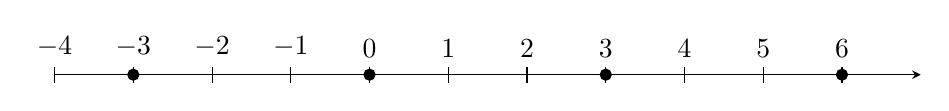
\begin{tikzpicture}
        \draw[-stealth] (-4,0) -- (7,0);
        \foreach \x in {-4,...,6}
            \draw (\x,-.1) -- (\x,.1) node[above]{$\x$};
        \foreach \y in {-3,0,...,6}
            \draw[fill=black] (\y,0) circle (2pt);
    \end{tikzpicture}
\end{figure}
Then any integer can be expressed by the closest left multiple of 3 and the amount of you have to travel right to reach it, for example 
\[
    5=3\times 1+2\hskip 32pt8=3\times 2+2
\]
We call the amount you walk to the right the remainder following division by 3.
\begin{theo}[Uniqueness of remainder]
    Let $d\in\mathbb{Z}$ where $d>0$, then $\forall x\in\mathbb{Z}$ there exists a unique remainder $r\in\mathbb{N}$ such that
    \[
        x=qd+r
    \]
    where $q\in\mathbb{Z}$ and $0\leq r<d$.
\end{theo}
\begin{prf}
    Assume that $x=q_{1}d+r_{1}$ and $n=q_{2}d+r_{2}$ where $q_{1},q_{2},r_{1},r_{2}\in\mathbb{Z}$ and $0\leq r_{1},r_{2}<d$ then
    \begin{align*}
        q_{1}d+r_{1}=q_{2}d+r_{2}&\implies q_{1}d-q_{2}d=r_{2}-r_{1} \\
                     &\implies d(q_{1}-q_{2})=r_{2}-r_{1}
    \end{align*}
    as we are assuming that $r_{1}\neq r_{2}$, we let $r_{2}$ be larger than $r_{1}$, which implies that $r_{2}-r_{1}=md$ where $m=q_{1}-q_{2}$, but this contradicts that $r_{2}-r_{1}\leq r_{2}<d$. To prove the existence of $r$, we let $M=\{x-qd~|~q\in\mathbb{Z}\}$, then $M\cap\mathbb{N}\neq\emptyset$, then $r$ must be the first element in $M\cap\mathbb{N}$, as such $\exists q,r=x-qd$, where $0\leq r<d$. If $r\geq d$ then $r>r-d\geq 0$ and $r-d=x-(q+1)d\in M\cap\mathbb{N}$, contradicting that $r$ is the first element in $M\cap\mathbb{N}$.
\end{prf}
\begin{defi}[Divisor]
    Suppose that $a=bc$ where $a,b,c\in\mathbb{Z}$, then we call $c$
    a divisor of $a$, which we write as $c\mid a$.
\end{defi}
\begin{defi}[Remainder]
    If $x,d\in\mathbb{Z}$ where $d>0$ we let $[x]_{d}$ be the unique remainder from Theorem 1.1.
\end{defi}
\pagebreak\subsection{Congruences}
\begin{defi}[Congruence]
    Let $a,b,c\in\mathbb{Z}$ then $a,b$ are called congruent modulo $c$ if $c\mid b-a$, denoted $a\equiv b\mod c$, which can be simply stated as them having the same remainder when divided by $c$.
\end{defi}
\begin{prop}[Congruence]
    Let $c\in\mathbb{Z}$ where $c>0$ then:
    \begin{itemize}
        \item[(i)] $a\equiv[a]_{c}\mod c$
        \item[(ii)] $a\equiv b\mod c\iff[a]_{c}=[b]_{c}$
    \end{itemize}
    for $a,b\in\mathbb{Z}$.
\end{prop}
\begin{prf}
    We know that $\exists q\in\mathbb{Z},a=qc+[a]_{c}$ by Theorem 1.1, whereby
    \begin{align*}
        a=qc+[a]_{c}&\implies a-[a]_{c}=qc \\
                    &\implies c\mid a-[a]_{c}=qc
    \end{align*}
    proving (i). We now define $b=q'c+[b]_{c}$ for some $q'\in\mathbb{Z}$, then
    \[
        a-b=(q-q')c+[a]_{c}-[b]_{c}
    \]
    whereby $c\mid a-b\iff c\mid[a]_{c}-[b]_{c}$ which as $0<[a]_{c},[b]_{c}<c\implies[a]_{c}=[b]_{c}$ proving (ii).
\end{prf}
\begin{prop}[Congruence of sum and product]
    Suppose that $x_{1}\equiv x_{2}\mod d$ and $y_{1}\equiv y_{2}\mod d$ then:
    \begin{itemize}
        \item[(i)] $x_{1}+y_{1}\equiv x_{2}+y_{2}\mod d$
        \item[(ii)] $x_{1}y_{1}\equiv x_{2}y_{2}\mod d$
    \end{itemize}
    for $x_{1},x_{2},y_{1},y_{2}\in\mathbb{Z}$.
\end{prop}
\begin{prf}
    Since $d$ divides $x_{1}-x_{2}$ and $y_{1}-y_{2}$, it must also divide the sum of the two
    \[
        d\mid x_{1}-x_{2}+y_{1}-y_{2}\implies d\mid x_{1}+y_{1}-(x_{2}+y_{2})
    \]
    proving (i). Similarly we recognize that
    \[
        x_{1}y_{1}-x_{2}y_{2}=x_{1}(y_{1}-y_{2})+y_{2}(x_{1}-x_{2})
    \]
    And as $x_{1},y_{2}$ are factors of terms we know to be divisible by $d$, so must their products be, and by (i) also their sum.
\end{prf}
\subsection{Greatest common divisor}
\begin{defi}[Divisor set]
    Let $\text{div}(n)=\{d\in\mathbb{N}~|~d\mid n\}$ be the set of natural divisors of $n\in\mathbb{Z}$.
\end{defi}

\subsection{Euclidean algorithm}
\subsection{Chinese remainder theorem}
